\documentclass{article}%
\usepackage[T1]{fontenc}%
\usepackage[utf8]{inputenc}%
\usepackage{lmodern}%
\usepackage{textcomp}%
\usepackage{lastpage}%
\usepackage[head=40pt,margin=0.5in,bottom=0.6in]{geometry}%
\usepackage{graphicx}%
%
\title{\textbf{Borrell reitera la importancia del regreso de Guaidó sin problemas}}%
\author{EFE}%
\date{04/03/2019}%
%
\begin{document}%
\normalsize%
\maketitle%
\textbf{URL: }%
http://www.el{-}nacional.com/noticias/europa/borrell{-}reitera{-}importancia{-}del{-}regreso{-}guaido{-}sin{-}problemas\_273302\newline%
%
\textbf{Periodico: }%
EN, %
ID: %
273302, %
Seccion: %
Europa\newline%
%
\textbf{Palabras Claves: }%
Europa, Mundo\newline%
%
\textbf{Derecho: }%
2.1%
, Otros Derechos: %
\newline%
%
\textbf{\textit{El presidente interino del país salió de Venezuela el pasado 22 de febrero para coordinar la entrada de la ayuda humanitaria}}%
\newline%
\newline%
%
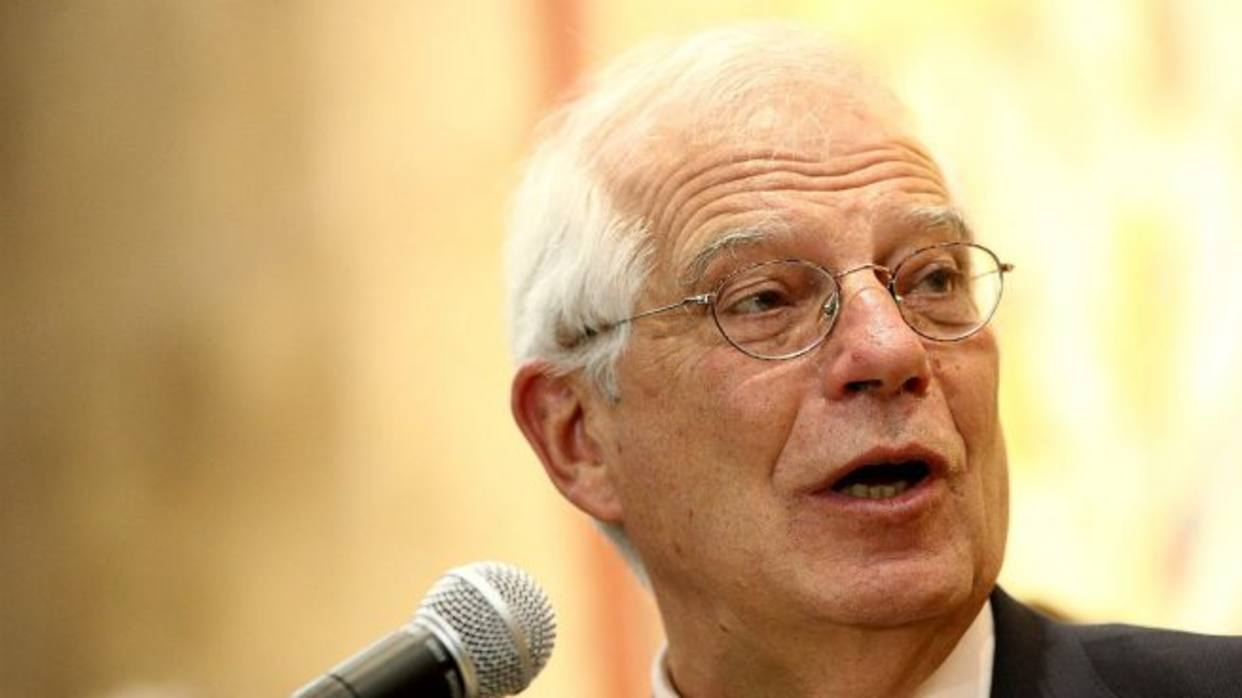
\includegraphics[width=300px]{EN_273302.jpg}%
\newline%
%
El ministro español de Asuntos Exteriores, Josep Borrell, reiteró este lunes la importancia de la advertencia que la Unión Europea le hizo a Nicolás Maduro~para que respete la capacidad del presidente de la Asamblea y presidente interino~del país, Juan Guaidó, de "ejercer libremente sus funciones".%
\newline%
%
En declaraciones a los medios, Borrell advirtió a~Maduro, de "las consecuencias, desde el punto de vista diplomático y de las relaciones" si "hubiera cualquier actuación contra el presidente interino de Venezuela".%
\newline%
%
El ministro español recordaba así el aviso que el pasado sábado hizo la UE contra cualquier acción que pudiese poner en peligro "la libertad, seguridad o integridad personal" del líder de la Asamblea Nacional de Venezuela, puesto que~incrementaría la tensión y merecería ser condenada.%
\newline%
%
Guaidó, quien salió de Venezuela el pasado 22 de febrero para coordinar la llegada de ayuda humanitaria a la frontera con Colombia y para realizar una gira internacional, ha anunciado que regreserá al país~este lunes y que confía en no tener problemas con las autoridades.%
\newline%
%
Las Justicia venezolana había prohibido el pasado 29 de enero que Guaidó saliera del país, además de otras medidas, como la congelación de sus cuentas, ante su "conducta delictiva", al declararse presidente interino de Venezuela.%
\newline%
%
"Señalamos la importancia que tiene que el señor Guaidó pueda ejercer libremente sus funciones de presidente de la Asamblea y, en nuestro caso, reconocido como presidente interino", subrayó~Borrell.%
\newline%
%
Preguntado por qué tipo de consecuencias internacionales tendría impedir el regreso de Guaidó a Caracas, Borrell aseguró que "las consecuencias pasan siempre por la actuación diplomática y la presión política".%
\newline%
%
La mayoría de los países de a UE han reconocido a Guaidó como "presidente interino" de Venezuela.%
\newline%
%
\end{document}